% mn2esample.tex
%
% v2.1 released 22nd May 2002 (G. Hutton)
%
% The mnsample.tex file has been amended to highlight
% the proper use of LaTeX2e code with the class file
% and using natbib cross-referencing. These changes
% do not reflect the original paper by A. V. Raveendran.
%
% Previous versions of this sample document were
% compatible with the LaTeX 2.09 style file mn.sty
% v1.2 released 5th September 1994 (M. Reed)
% v1.1 released 18th July 1994
% v1.0 released 28th January 1994

\documentclass[useAMS,usenatbib]{mn2e}
\usepackage[T1]{fontenc}
\usepackage{prettyref}
\usepackage{amsmath}
\usepackage{graphicx}
\usepackage{subfigure}
\usepackage{epstopdf}
\usepackage{color}
\usepackage[breaklinks=true]{hyperref}  

% If your system does not have the AMS fonts version 2.0 installed, then
% remove the useAMS option.
%
% useAMS allows you to obtain upright Greek characters.
% e.g. \umu, \upi etc.  See the section on "Upright Greek characters" in
% this guide for further information.
%
% If you are using AMS 2.0 fonts, bold math letters/symbols are available
% at a larger range of sizes for NFSS release 1 and 2 (using \boldmath or
% preferably \bmath).
%
% The usenatbib command allows the use of Patrick Daly's natbib.sty for
% cross-referencing.
%
% If you wish to typeset the paper in Times font (if you do not have the
% PostScript Type 1 Computer Modern fonts you will need to do this to get
% smoother fonts in a PDF file) then uncomment the next line
% \usepackage{Times}

%%%%% AUTHORS - PLACE YOUR OWN MACROS HERE %%%%%

\title[Results of two stellar occultations by Ceres]{Results of two multi-chord stellar occultations by dwarf planet (1) Ceres}
\author[A. R. Gomes-J\'unior, B. L. Giacchini, F. Braga-Ribas et al.]{A. R. Gomes-J\'unior$^{1,}$\thanks{E-mail: altair08@astro.ufrj.br},
B. L. Giacchini$^{2,3,4}$,%\thanks{E-mail: breno@cbpf.br},
F. Braga-Ribas$^{5, 6, \dag}$,
M. Assafin$^{1, \dag, \ddag}$,\newauthor
R. Vieira-Martins$^{1,5, \dag, \ddag}$,
J.I.B. Camargo$^{5, \dag}$,
B. Sicardy$^{7}$,
B. Timerson$^{4}$, 
T. George$^{4}$, \newauthor
J. Broughton$^{8}$, 
T. Blank$^{4}$,
G. Benedetti-Rossi$^{5}$, 
J. Brooks$^{4}$,  
R. F. Dantowitz$^{9}$,  \newauthor
D. W. Dunham$^{4}$, 
J. B. Dunham$^{4}$, 
C. K. Ellington$^{4}$,
M. Emilio$^{10}$,
F.R. Herpich$^{11}$,  \newauthor
C. Jacques$^{3, 12}$,
P. D. Maley$^{4,13}$,
L. Mehret$^{10}$,
A.J.T. Mello$^{14}$,
A.C. Milone$^{15}$,\newauthor
E. Pimentel$^{3, 12}$,  
W. Schoenell$^{11}$,
N. S. Weber$^{9}$
\\
$^{1}$Observat\'orio do Valongo/UFRJ, Ladeira Pedro Ant\^onio 43,
CEP 20.080-090 Rio de Janeiro - RJ, Brazil\\
$^{2}$Centro Brasileiro de Pesquisas F\'isicas, Rua Dr. Xavier Sigaud 150, Rio de Janeiro  22290-180, Brazil\\
$^{3}$Se\c{c}\~ao de Oculta\c{c}\~oes/REA-Brasil, Belo Horizonte, Brazil\\
$^{4}$International Occultation Timing Association, P.O. Box 131034, Houston, TX 77219-1034, USA\\
$^{5}$Observat\'orio Nacional/MCTI, R. General Jos\'e Cristino 77, CEP 20921-400 Rio de Janeiro - RJ, Brazil\\
$^{6}$Federal University of Technology - Paran\'a (UTFPR / DAFIS), Rua Sete de Setembro, 3165, CEP 80230-901, Curitiba, PR, Brazil\\
$^{7}$LESIA, Observatoire de Paris, CNRS UMR 8109, Universit\'{e} Pierre et Marie Curie, Universit\'{e} Paris-Diderot, 5 place Jules Janssen,\\ F-92195 Meudon Cedex, France\\
$^{8}$RASNZ Occultation Section, P.O. Box 3181, Wellington, New Zealand\\
$^{9}$Clay Center Observatory at Dexter Southfield, 20 Newton Street, Brookline, MA 02445, USA\\
$^{10}$Universidade Estadual de Ponta Grossa, Ponta Grossa, Brazil\\
$^{11}$Universidade Federal de Santa Catarina, Florian\'opolis, Brazil\\
$^{12}$Centro de Estudos Astron\^omicos de Minas Gerais, Belo Horizonte, Brazil\\
$^{13}$NASA Johnson Space Center Astronomical Society, Houston, Texas, USA\\
$^{14}$Federal University of Technology - Paran\'a (UTFPR / DAELT), Rua Sete de Setembro, 3165, CEP 80230-901, Curitiba, PR, Brazil\\
$^{15}$Instituto Nacional de Pesquisas Espaciais, S\~ao Jos\'e dos Campos, Brazil\\
$^\dag$ Associated to Laborat\'{o}rio Interinstitucional de e-Astronomia - LIneA, Rua Gal. Jos\'e Cristino 77, CEP 20921-400,\\ Rio de Janeiro, Brazil\\
$^\ddag$Affiliated researcher at Observatoire de Paris/IMCCE, 77 Avenue Denfert Rochereau 75014 Paris, France
}
\begin{document}

\date{Accepted . Received ; in original form }

\pagerange{\pageref{firstpage}--\pageref{lastpage}} \pubyear{2015}

\maketitle

\label{firstpage}

\begin{abstract}
We report the results of two multi-chord stellar occultations by the dwarf planet (1) Ceres that were observed  from Brazil on 2010 August 17, and from the USA on 2013 October 25. Four positive detections were obtained for the 2010 occultation, and nine for the 2013 occultation. Elliptical models were adjusted to the observed chords to obtain Ceres' size and shape. Two limb fitting solutions were studied for each event. The first one is a nominal solution with an indeterminate polar aspect angle. The second one was constrained by the pole coordinates as given by Drummond et al. Assuming a Maclaurin spheroid, we determine an equatorial diameter of 972 $\pm$ 6 km and an apparent oblateness of $0.08 \pm 0.03$ as our best solution. These results are compared to all available size and shape determinations for Ceres made so far, and shall be confirmed by the NASA's \textit{Dawn} space mission.
\end{abstract}

\begin{keywords}
minor planets, asteroids: individual (1, Ceres) - occultations - planets and satellites: fundamental parameters
\end{keywords}

\section{Introduction}

Ceres is the sole example of a dwarf planet in the inner Solar System. Far from being mere taxonomic information, this suggests the great impact its study can have on the understanding of planetary formation and evolution of the Solar System. Indeed, it was proposed that Ceres' origin could have been as a transneptunian object \citep{McKinnon12}, later scattered to the Main Belt due to the giant planets' migration predicted by the `Nice Model' \citep{Gomes05}. Even if it was formed close to its current location, the dynamical history of the Solar System must have let its signatures on Ceres. These could include not only the late heavy bombardment features that might exist on its surface, but also the makeup of its volatiles, which could have been transported from the outer region.

Since the 1970's it has been speculated that Ceres could contain water ice, which was recently verified \citep{Kuppers2014}. Although the water regime on this object is still unknown, some internal structure models suggest the existence of a water ice -- or even a liquid water -- layer \citep{CastilloR2011}. Yet the very question of whether Ceres underwent differentiation is open and, on the assumption of an affirmative answer, it is natural to ask if it ever had tectonics, what its geological evolution was, and if it is still active. Inarguably NASA's \textit{Dawn} mission \citep{Russell2004}, which is currently orbiting the dwarf planet, will shed light on several open issues concerning Ceres.

Containing approximately one fifth of the whole Main Belt's mass, Ceres is expected to have an equilibrium figure, i.e. a Maclaurin or a Jacobi ellipsoid. In fact, direct observations of Ceres by means of adaptive optics indicate that it is an oblate spheroid \citep{Drummond2014}. The precise knowledge of its size and shape is of utmost importance, for the models of density, internal structure and differentiation.% can depend on the size and oblateness of the body.

The best ground-based technique for determining shape and size of a faraway object is the study of its shadow, cast by a star during an occultation. Since the 1960's occultations have provided measurements of hundreds of asteroids, thanks partially to the fruitful professional-amateur collaboration on the field. More recently, this technique has been applied to objects of the outer Solar System and has unveiled outstanding features of distant bodies, e.g. the ring system around the Centaur (10199) Chariklo \citep{BragaRibas2014}.

The first stellar occultation by Ceres was observed in 1984 \citep{Millis1987} and led to the determination of its size to the precision of some kilometres, at a time when the uncertainties were often ten times larger. The high apparent brightness of Ceres, as compared to most asteroids, imposes a somewhat strong constraint on the stars capable of causing a detectable magnitude drop when occulted. For instance, after the 1984 event, to our knowledge, only four stellar occultations have been observed \citep{Dunham2014}. Two of them had only two chords each, thus not sufficient for providing accurate results\footnote{These events took place on 1994 August 22 and 2010 October 30.}. The two remaining events, which occurred on 2010 August 17 and 2013 October 25, are reported in the present work and are the first ones that used charged-couple devices (CCD) as recording systems. % The former was observed in Brazil from 4 stations, while the latter was from the United States and led to 9 chords.
Throughout the paper we shall refer to these events as the `2010 occultation' and the `2013 occultation'.

Both events were predicted by Steve Preston\footnote{Predictions are published at http://asteroidoccultation.com.} on behalf of the International Occultation Timing Association, during routine prediction of asteroidal occultations of bright stars.

This work is organized as follows. In Sections 2 and 3 we analyse the 2010 and the 2013 occultations, respectively. In Section 4 we give the geocentric positions of Ceres derived from the occultations. The comparison of our results to those in the literature is carried out in Section 5.



\section{The 2010 occultation}

\subsection{Observations}


As predicted, on 2010 August 17 Ceres occulted the star TYC 6833-163-1 (UCAC4 313-111823), which has magnitude $V = 11.55$ and has the ICRS position, based on UCAC4 catalogue \citep{Zacharias2013}, to the date of occultation:

%abaixo (UCAC2 20678706),
\begin{equation}
\left\{ 
  \begin{array}{l l}
    \alpha = 17^{\rmn{h}}18^{\rmn{m}}29\fs0085\\
    \delta = -27\degr 26\arcmin 38\farcs 867
  \end{array}
\right.
\label{Eq: 2010-coord}
\end{equation}

% Abaixo a coordenada UCAC4 aplicada de Movimento Próprio
% UCAC4 313-111823
%
%\begin{equation}
%\left\{ 
%  \begin{array}{l l}
%    \alpha = 17^{\text{h}}18^{\text{m}}29^{\text{s}}.009\\
%    \delta = -27\degr 26\arcmin 38\arcsec.866.
%  \end{array}
%\right.
%\label{Eq: 2010-coord}
%\end{equation}
%
%The shadow's path would cross South America, the Atlantic and reach the south part of Africa.

\begin{figure}
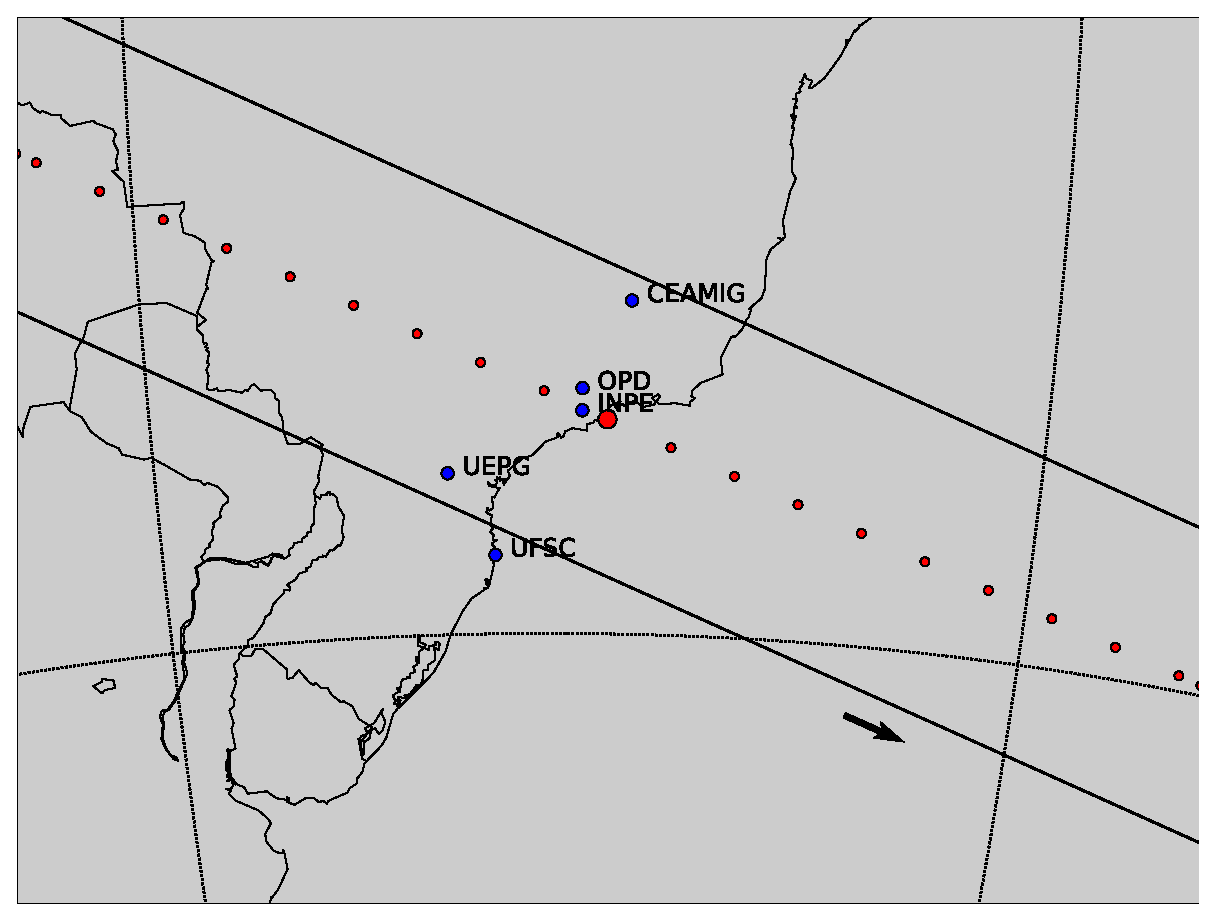
\includegraphics[scale=0.42]{figures/Ceres_2010.eps} 
\caption{Post-occultation reconstruction of Ceres' shadow path on Earth for the 2010 August 17 event. The big red dot is the geocentric closest approach at 22:40:25 UT. The small red ones represent the centre of the shadow separated by one minute, shadow moves from the left to the right. Blue dots are the sites that have observed the event. As described in text, UFSC had a negative chord.
\label{Fig: Ceres-2010-map}}
\end{figure}

Observations were carried out in Brazil from five different sites as displayed in Table \ref{Tab: obs-2010} and Fig. \ref{Fig: Ceres-2010-map}. The occultation was detected from four of them. The southern-most one (UFSC) had a negative chord. From the positive sites, the one named INPE started observing after the event was already in progress, due to technical difficulties, thus providing only the star's reappearance time; the other three recorded the whole phenomenon.

A remarkable circumstance of this event was the low velocity of Ceres: only 3.9 km s$^{-1}$ in the plane of the sky. Therefore, even exposures of a few seconds would translate in a relevant spatial resolution.

All the observations were made through a sequence of images obtained with CCDs. The times of each exposure were available on the header of each image with an internal accuracy of a few hundredths of a second. CEAMIG had only the integer part of the second available, due to the acquisition software used. The fraction of a second could be retrieved as described on the Section~3.1 of \cite{BragaRibas2013}  (which shall be referred as BR13 hereafter). Cycle times (exposure plus read-out) varied from 2 to 52 seconds, as can be verified on Table~\ref{Tab: obs-2010}, making it a heterogeneous set of observations and imposing an error of a few seconds for the ingress / egress times of some sites.


%\textcolor{blue}{[Falar sobre a quest\~ao do tempo em cada corda. A leitura do header era no segundo inteiro? Foi analisada a cad\^encia das imagens? Qual a precis\~ao?] [Durante o per\'iodo de observac\~ao Ceres rodou apenas 3.1$\degr$. Mas isso n\~ao \'e relevante no caso de Maclaurin...]}

\begin{table*}
 \centering
 \begin{minipage}{140mm}
  \caption{Circumstances of observation for all observing stations of the 2010 event. \label{Tab: obs-2010}}
  \begin{tabular}{@{}lccccc}
  \hline
          & Longitude & Telescope & Exposure & Result &   \\
     Site & Latitude  & Aperture  & Cycle time & Ingress & Observer\\          
          & Height    & f-ratio & Camera & Egress    & \\          
\hline
 Belo Horizonte & 43$\degr$59\arcmin 51\farcs1~W & LX200 & 5 s & Positive & C. Jacques  \\
 CEAMIG-REA &19$\degr$49\arcmin 49\farcs0~S & 31 cm & 12 s & 22:39:03.9 $\pm$ 0.6 s &  E. Pimentel \\
            & 825 m       &  f/10         &   SBIG ST10        & 22:40:20 $\pm$ 5 s &   \\
 & & & & & \\
 Pico dos Dias    & 45$\degr$34\arcmin45\farcs1~W &  Zeiss     & 1 s & Positive & J. I. B. Camargo \\
 LNA    &22$\degr$32\arcmin03\farcs7~S & 60 cm & 2 s & 22:37:30.3 $\pm$ 0.6 s &  G. B. Rossi \\
            & 1864 m     & f/12.5          &    Andor Ikon       & 22:41:55.3 $\pm$ 0.7 s &              \\
 & & & & & \\
 S\~ao Jos\'e dos       & 45$\degr$51\arcmin44\farcs0~W &  C11  & 2 s & Egress only & A. C. Milone\\
 Campos       &23$\degr$12\arcmin33\farcs0~S & 28 cm & 5 s & Start obs.: 22:39:44 & T. Maldonado\\
 INPE      & 620 m      & f/6.3          & SBIG ST7     & 22:42:03.0 $\pm$ 0.2 s & M. Okada    \\
 & & & & & \\
 Ponta Grossa       & 50$\degr$05\arcmin56\farcs0~W & RCX 400 &30 s & Positive & M. Emilio   \\
 UEPG       &25$\degr$05\arcmin22\farcs2~S & 40 cm & 52 s & 22:37:17 $\pm$ 13 s & L. Mehret   \\
            & 910 m      & f/8          & SBIG STL6E     & 22:39:56 $\pm$ 13 s & \\
 & & & & & \\
 Florian\'opolis       & 48$\degr$31\arcmin20\farcs5~W &   C11      & 3 s & No occultation  & W. Schoenell\\
 UFSC       &27$\degr$36\arcmin12\farcs3~S & 28 cm & 6 s&  Start obs.: 21:49:27 & A. J. T. Mello\\
            & 20 m       & f/10          &  SBIG ST7      &   End obs.: 22:51:21      & F. R. Herpich \\
\hline
\end{tabular}
\end{minipage}
\end{table*}




\subsection{Light curves \label{Sec: light-curve-2010}}

The flux of the star in the five occultation chords was obtained from the FITS images with the \textsc{platform for reduction of astronomical images automatically (praia)} \citep{2011gfun.conf...85A}. The light curves were normalized to the flux of the star plus Ceres, as they were merged right before and after the occultation. Additionally,
%, with exception of INPE
 they were normalized by fitting a polynomial curve (of first or second order) outside the flux drop, so that the flux ratio was set to 1 outside the occultation.

The ingress (disappearance) and egress (reappearance) instants of the occultation were obtained for each light curve by fitting a square-well model convoluted with the Fresnel diffraction, the CCD bandwidth, the stellar apparent diameter, and the applied finite exposure time; see \cite{Widemann2009} and BR13. %\cite{BragaRibas2013}.
%The Fresnel scale ($F = \sqrt{\lambda D/2}$) for the present Ceres' geocentric distance $D = 2.29 \text{ au} = 3.42 \times 10^{8}$~km is 0.3~km for a typical wavelength of $\lambda = 0.65$~$\micron$. The star diameter is estimated using the formulae of \cite{vanBelle1999}. Its $B$, $V$, and $K$ apparent magnitudes are 12.00, 11.78 and 9.18, respectively, in the Tycho catalog \citep{Hog2000}. This yields a diameter of about 0.11~km projected at Ceres' distance. 
The smallest integration time used in the positive observations was 1.0~s, which translates to almost 3.9 km in the celestial plane. Therefore, the error on the time determination of the ingress and egress is largely dominated by the integration times, not by Fresnel diffraction or star diameter, which are both on the order of a few hundred meters for this event.
The occultation data fit consists in minimizing a classical $\chi^{2}$ function for each light curve, as described in \cite{Sicardy2011} and BR13.\ The free parameter to adjust is the ingress or egress instant, which provides the minimum value of $\chi^{2}$, denoted as $\chi^{2}_{min}$. The best fittings to the 2010 occultation light curves are shown in Fig. \ref{Fig: Ceres-2010-curves}, and the derived occultation times are listed in Table~\ref{Tab: obs-2010}.
%The occultation fits consist in minimizing a classical $\chi^{2}$ function for each light curve, as described in \cite{Sicardy2011} and BR13.\ The free parameter to adjust is the ingress (disappearance) or egress (reappearance) time $t_{occ}$, which provides the minimum value of $\chi^{2}$, denoted as $\chi^{2}_{min}$. The best fittings to the 2010 occultation light curves are shown in Fig. \ref{Fig: Ceres-2010-curves}, and the derived occultation times are listed in Table~\ref{Tab: obs-2010}.


\begin{figure}
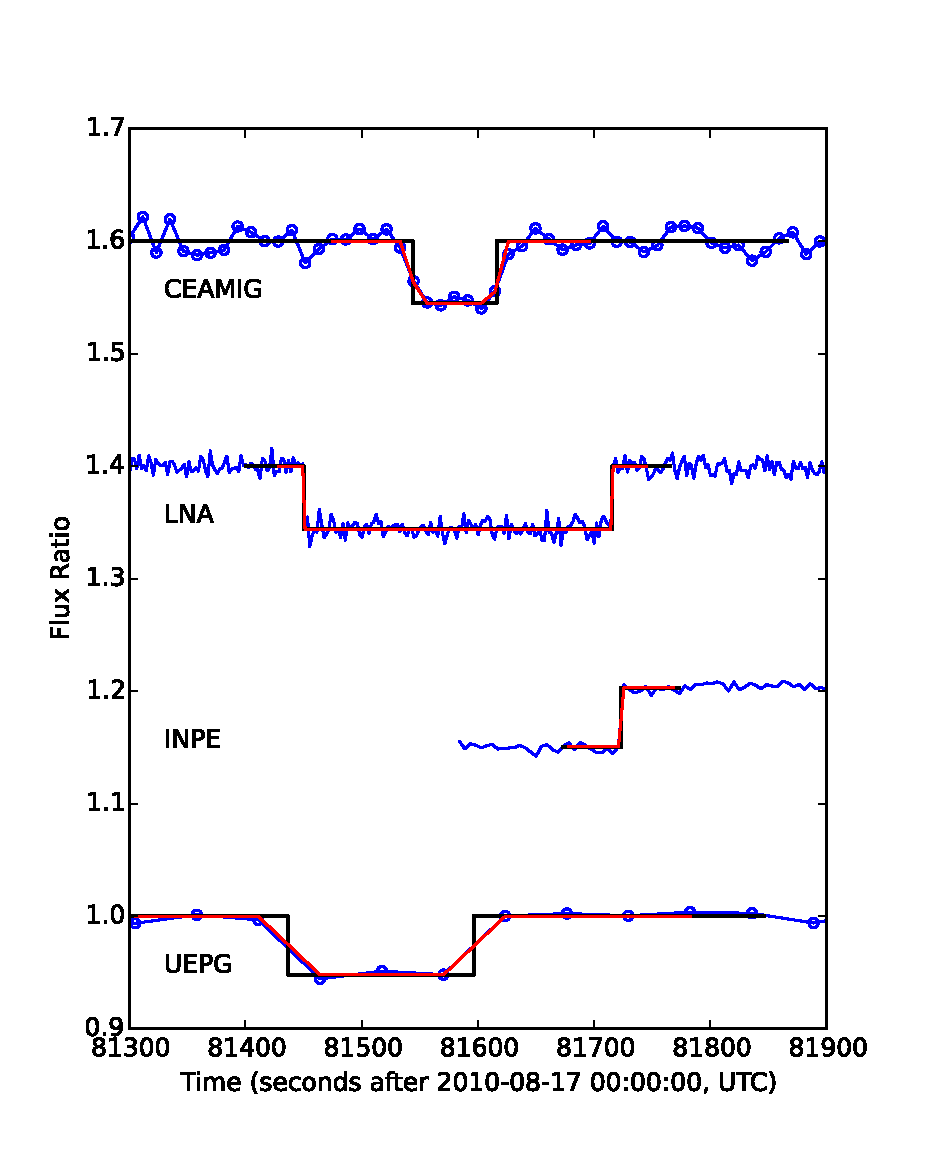
\includegraphics[scale=0.58]{figures/Ceres_2010_fluxratio.eps} 
\caption{The four occultation light curves normalized and vertically shifted by a factor of 0.2 for better visualisation. The solid black lines are the best fit of the square-well model to the data. Red lines are the square-well model convoluted with the Fresnel diffraction, the star diameter, and the applied exposure time. The mid-times of the occultations do not coincide due to the propagation delays of the shadow due to the distinct longitude of the sites. Exposures at INPE started after the immersion, as explained in the text. \label{Fig: Ceres-2010-curves}}
\end{figure}


\subsection{Limb fitting methodology} \label{Sec: limbfittingmethod}

The methodology used to analyse Ceres' profile from the observations is the same described by \cite{Sicardy2011} and BR13.%\cite{BragaRibas2013}. 
 ~Each combination of site position and recorded ingress/egress instant, together with star coordinates and Ceres' ephemeris, corresponds to a point in the plane of the sky. The collection of all these points ideally determines the apparent limb of Ceres.
%~To each combination of site position and recorded ingress/egress time, together with star coordinates and Ceres' ephemeris, corresponds a point $(f_{i,obs},g_{i,obs})$ on the plane of the sky. The collection of those points ideally determines the apparent limb of Ceres.


We adopt an elliptic model for the limb profile, resulting from the projection of an oblate spheroid onto the sky plane. This choice is supported by the work of \cite{Drummond2014}, by means of direct imaging of Ceres. Hence, we have $N=7$ chord extremities to adjust the $M=5$ parameters which define an ellipse: apparent semimajor and semiminor axis ($a^\prime$ and $b^\prime$, respectively), position angle $P$ of its semiminor axis and the position $(f_c,g_c)$ of its centre with respect to the occulted star. 
Of course, the apparent semimajor axis {$a^\prime$} is equivalent to the equatorial radius $R_{equa}$ of the ellipsoid.
The coordinates $f_{c}$ and $g_{c}$, in kilometres, are calculated using the JPL\#33 Ceres' ephemeris \citep{Giorgini1996} and the occulted star's position. They are positive toward the local celestial east and north, respectively. The position angle $P$ is counted positively from the direction of local celestial north to celestial east. The apparent oblateness can be defined by $\epsilon^\prime = 1 - (b^\prime/a^\prime)$. The best-fitting solution is obtained minimizing a reduced $\chi^{2}_{r}$ function, where we define the number of degrees of freedom of the problem as $\mathcal{N} \equiv N - M$.  All the procedures that allow the determination of the error bars of the physical parameters can be found on BR13.

%We adopt an elliptic model for the limb profile, resulting from the projection of an oblate spheroid onto the sky plane. This model is supported by the work of \cite{Drummond2014}, by means of direct imaging of Ceres. Hence, we have $N=7$ chord extremities to adjust the $M=5$ parameters which define an ellipse: apparent semimajor and semiminor axis -- $a^\prime$ and $b^\prime$, respectively --, position angle $P$ of its semiminor axis and the position $(f_c,g_c)$ of its centre with respect to the occulted star\footnote{The coordinates $f_{c}$ and $g_{c}$, in kilometres, are calculated using the JPL\#33 Ceres' ephemeris and the occulted star's position. They are positive toward the local celestial east and north, respectively. The position angle $P$ is counted positively from the direction of local celestial north to celestial east.}. The first two parameters can be interchanged with the oblateness and the equivalent radius, defined, on this order, by $\epsilon^\prime = 1 - (b^\prime/a^\prime)$ and $R_{equiv} \equiv \sqrt{a^\prime b^\prime} = a^\prime\sqrt{1-\epsilon^\prime}$. We define the number of degrees of freedom of the problem as $\mathcal{N} \equiv N - M$.

%%The apparent oblateness is related to the true one $\epsilon$ through
%%%
%%\begin{equation}
%%\epsilon^\prime = 1 - \sqrt{\cos^2(\zeta) + (1-\epsilon)^2\sin^2(\zeta)},
%%\label{Eq: TrueObla}
%%\end{equation}
%%%
%%where $\zeta$ is the polar aspect angle, encompassed by the (true) polar semiminor axis and the line of sight. Of course, the apparent semimajor axis $a^\prime$ equals the equatorial radius $R_{equa}$ of the ellipsoid.
%%
%%%Correspondence between true and apparent figures depends on the polar aspect angle $\zeta$, encompassed by the (true) polar $b$-axis and the line of sight. The apparent oblateness is related to the true one, $\epsilon$, through
%%
%%The search for the best-fitting ellipse is carried out by minimizing the reduced $\chi^2$ function:
%%%
%%\begin{equation}
%%\chi^2_r = \frac{1}{\mathcal{N}} \sum_{i=1}^N \frac{1}{\sigma_i^2}  \left[ (f_{i,obs}-f_{i,cal})^2 + (g_{i,obs}-g_{i,cal})^2\right].
%%\end{equation}
%%%
%%Here $\sigma_i$ is the radial uncertainty of the $i$th chord extremity, obtained by multiplying the time uncertainty reported in Table~1 by the normal velocity of the star (with respect to the limb model). $f_{i,cal}$ and $g_{i,cal}$ are the coordinates of the point on the model ellipse, where a line that goes from the centre of the model to the data point $(f_{i,obs},g_{i,obs})$ intersects the ellipse.%:
%%%
%%%\begin{equation}
%%%f_{i,cal} \equiv f_{i,obs} + \rho \cos(\theta), \quad g_{i,cal} \equiv %g_{i,obs} + \rho \sin(\theta),
%%%\end{equation}
%%%
%%%with:
%%%\begin{equation}
%%%\theta \equiv \arctan\left( \frac{g_{i,obs}-g_{c}}{f_{i,obs}-f_{c}} %\right) ,
%%%\end{equation}
%%%
%%%\begin{equation}
%%%\rho \equiv a^\prime b^\prime / \sqrt{[a^\prime\sin(\theta+P)]^2 +[b^\prime\cos(\theta+P)]^2 }.
%%%\end{equation}
%%
%%Evaluation of the reduced $\chi^2$ function over the $\lbrace R_{equa}, \epsilon^\prime, P, f_c, g_c \rbrace$--space produces a map related to the likelihood of a solution. For instance, the 1--sigma reported time uncertainties correspond to the subset of the parameter space for which $\chi^2_r$ lies between ${\chi^2_r}_{min}$ and ${\chi^2_r}_{min} + 1$. This allows the determination of the error bars of the physical parameters. It is worthwhile to mention that we consider all the uncertainty as due to timing issues.





\subsection{Limb fitting solutions}\label{Sec: limbfitting-2010}

Two possible solutions were considered for the limb fitting. The first, which we call nominal solution, consists of determining the five parameters that characterize an ellipse from the seven observed contacts. As we shortly show, it led to a rather large uncertainty on the position angle. Furthermore, the nominal solution alone is not capable of returning the true oblateness, which can be evaluated through equation 2 of BR13  provided that the aspect angle $\zeta$ is known.% or constrained by some physical hypothesis.

From observations with adaptive optics spanning a 10-year period, \cite{Drummond2014} determined the position of Ceres' polar axis within an error of only 3$\degr$:
\begin{equation}
%\left\{ 
%\begin{array}{l}
\alpha = (287 \pm 3) \degr, \quad %\\
\delta = (+64 \pm 3) \degr,
%\end{array} \right .
\label{Eq: Pole}
\end{equation}
%
in equatorial J2000 coordinates. Together with Ceres' ephemeris at the moment of the occultation, this corresponds to the polar aspect angle $\zeta = 86.1\degr$, which is very close to an equator-on geometry. Hence, we expect true figures to be similar to apparent ones.

The knowledge of Ceres' pole not only allows the determination of its polar aspect, it suffices to set its position angle. Therefore Eq.~\ref{Eq: Pole} may act as a constraint for $P$, and a second solution can be obtained by probing the parameter space with the restriction that the position angle is confined to the range that follows from Eq.~\ref{Eq: Pole}. We call this the `pole-constrained solution'.


\subsubsection{Nominal solution}

With the seven observed contacts it is possible to adjust the five parameters which define an ellipse. For the best-fitting solution we find $\chi^2_{r,min} = 0.24$, which could be interpreted as a slightly overestimation of the error bars with regard to the good quality of the fit. However, inasmuch as the problem has only two degrees of freedom, it is far from the statistical realm and relatively small $\chi^2_{r,min}$ are acceptable.

The resulting values of equatorial diameter, oblateness, position angle and centre coordinates are presented in the second column of Table~\ref{Tab: results}.%, and the corresponding ellipse is plotted with the observed chords in Fig.~2.
% The equivalent radius of the best-fitting solution is $R_{equiv} = 469 \pm 10$ km.

Already mentioned, the parameter with the largest uncertainty is the position angle: spanning on a 20$\degr$ interval, its determination has a relative precision worse than 10 per cent. Clearly, the coordinates of Ceres' pole (Eq. \ref{Eq: Pole}) can impose a strong constraint on the position angle, as the next solution shows.

Finally, the correction to the oblateness due to Ceres' polar aspect angle lies within the 1-sigma error bar and has no statistical relevance; hence $\epsilon = 0.08 \pm 0.03$.





\subsubsection{Pole-constrained solution}

At the occultation, the coordinates (Eq. \ref{Eq: Pole}) of Ceres' rotational pole correspond to the position angle $P = (12 \pm 3)\degr$. Exploration of the parameter space, restricted to ellipses with position angles laying within this range, results in the pole-constrained solution. The related physical parameters are displayed on the third column of Table \ref{Tab: results} in boldface, while the best-fitting solution is depicted in Fig.\ref{Fig:Ceres-2010-body}.

We notice that the constraint corresponds to the upper limit of nominal solution's 1-sigma error bar for $P$. On the other hand, it selects the smallest values of semimajor axis, improving its determination by a factor of about 2. Notwithstanding, oblateness' figures remain the same.


\begin{table*}
 \centering
 \begin{minipage}{140mm}
  \caption{Results of limb fitting to the data of the 2010 and 2013 events.\label{Tab: results}}
  \begin{tabular}{@{}lcccc}
  \hline
     Solution & 2010/Nominal & \textbf{2010/Pole-constrained} & 2013/Nominal & 2013/Pole-constrained \\
\hline
Equatorial diameter (km) & 982 $\pm$ 14 & \textbf{972 $\pm$ 6}  & 971 $\pm$ 7  & 971 $\pm$ 7\\
%Equatorial radius (km) & 491 $\pm$ 7  & \textbf{486 $\pm$ 3}  & 485.5 $\pm$ 3.5 & 485.5 $\pm$ 3.5\\
True oblateness        & 0.08 $\pm$ 0.03 & \textbf{0.08 $\pm$ 0.03} & 0.08 $\pm$ 0.04 & 0.08 $\pm$ 0.04\\
Position angle (deg)   & 5 $\pm$ 10    & \textbf{12 $\pm$ 3} (*)& 22 $\pm$ 5    & 25 $\pm$ 3 (*)\\
$f_c$ (km)             & 97 $\pm$ 9   & \textbf{102 $\pm$ 5}   & 77 $\pm$ 6    & 78 $\pm$ 6\\
$g_c$ (km)             & 16 $\pm$ 15  & \textbf{21 $\pm$ 11}  & 13 $\pm$ 16   & 13 $\pm$ 16\\
$\chi^2_{r,min}$       & 0.24          &  \textbf{0.42}         & 1.27          & 1.27\\
\hline
\end{tabular}
\textbf{Notes.} In bold we highlight our best solution. Error bars are at 1-sigma level. The polar diameter ($D_{pol}$) can be easily calculated from $D_{pol}=D_{equa}(1 - \epsilon)$.
(*) Position angle derived from Ceres' rotational pole coordinates determined by \cite{Drummond2014}.
\end{minipage}
\end{table*}

\begin{figure}
\includegraphics[scale=0.37, angle=-90]{figures/Ceres_2010_sphere.eps} 
\caption{The best elliptical fit for the occultation chords for the event of 2010 using the times from Table~\ref{Tab: obs-2010} and the pole-constrained solution. The arrow indicates the direction of motion, blue lines are the observed chords, the red segments are the ingress, egress and mid-occultation error bars at 1-$\sigma$ level. \label{Fig:Ceres-2010-body}}
\end{figure}







\section{The 2013 occultation}

\subsection{Observations}\label{Sec: observation-2013}

The event which took place on 2013 October 25 involved the star TYC 865-911-1 (UCAC4 496-058191), of magnitude $V = 10.05$. Based on UCAC4 \citep{Zacharias2013}, the ICRS position to the date of occultation is:
%
\begin{equation}
\left\{ 
  \begin{array}{l l}
    \alpha = 11^{\rmn{h}}57^{\rmn{m}}52\fs7641\\
    \delta = +09\degr 07\arcmin 49\farcs835
  \end{array}
\right.
\end{equation}
%
The occultation could only be visible in the United States, before dawn, as depicted in Fig. \ref{Fig: Ceres-2013-map}.% The shadow would then cross the Atlantic and Africa, but during daylight time.

\begin{figure}
%\begin{centering}
%\subfigure{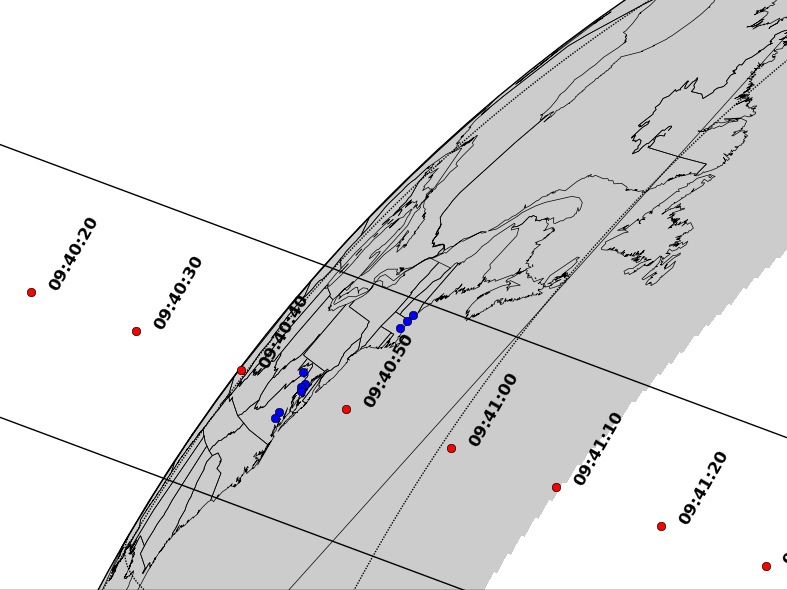
\includegraphics[scale=0.42]{figures/Ceres_2013_2.png}}
%\hspace{5mm}
%\subfigure
{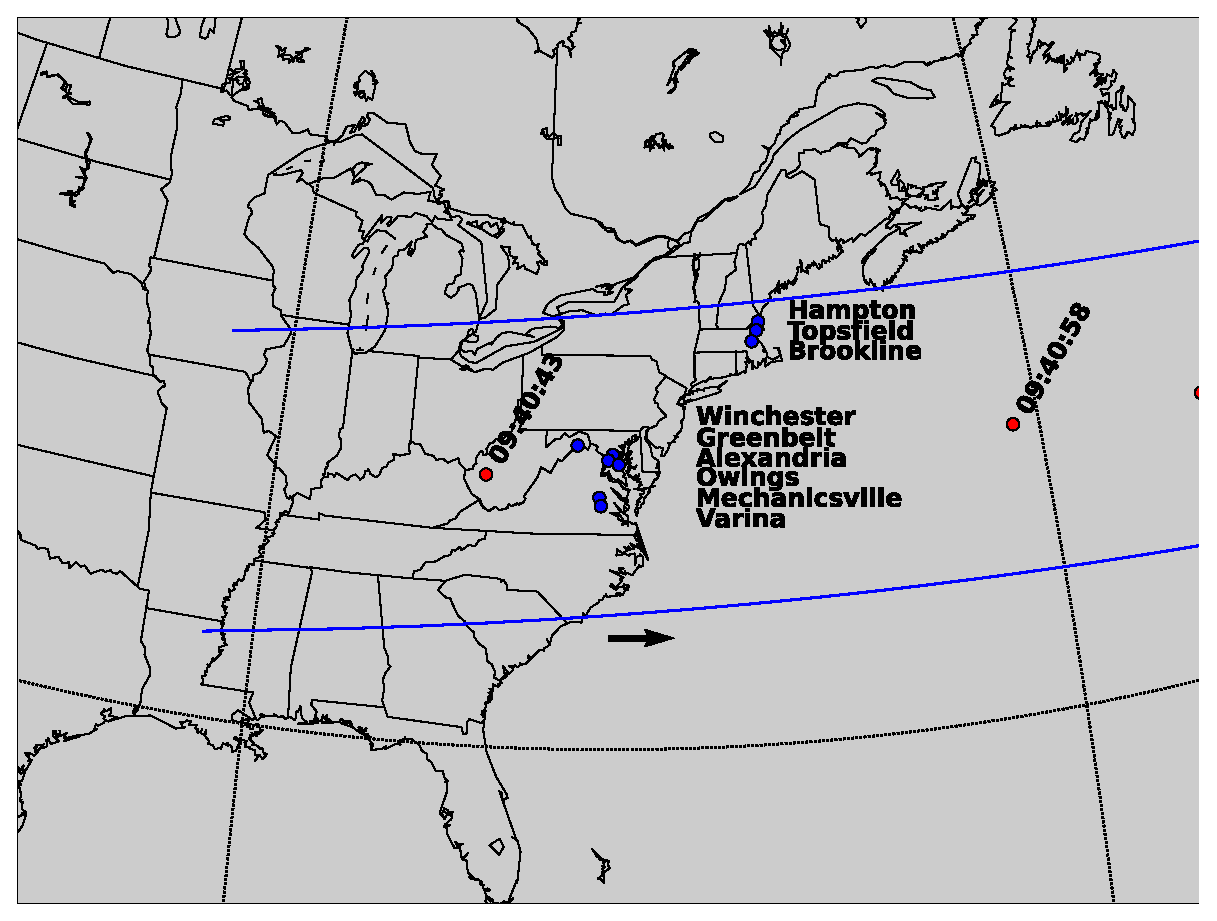
\includegraphics[scale=0.42]{figures/Ceres_2013-zoom.eps}}
\caption{Post-occultation reconstruction of Ceres' shadow path on Earth for the 2013 October 25 event at the east coast of USA. 
%Left panel: Overview of the occultation. The big red dot is the geocentric closest approach at 09:43:03 UT and the small ones represent the centre of the shadow separated by 30 seconds where the shadow moves from the left to the right. The blue dots are the sites that have observed the event. 
Upper view of the occultation over the sites that observed the event (blue dots). Red points are the centre of the shadow separated by 15 seconds.
\label{Fig: Ceres-2013-map}}
%\end{centering}
\end{figure}

Nine positive chords were obtained by the variety of instruments listed in Table \ref{Tab: obs-2013}. Each station was equipped with a video camera with negligible readout times. This was of particular importance, since in this event Ceres' shadow speed was 42.6 km s$^{-1}$, much faster than in the 2010 event.

Three different timing synchronization procedures were adopted among the set of observing stations. At Greenbelt and Owings the 1PPS signal of a GPS unit was used to calibrate time stamps which were inserted at each frame of the video. Time extraction is thus straightforward, after taking camera delays into account. On the other hand, at Brookline the clock would be synchronized by an internet server. A lack of connection, however, resulted in spurious times. In fact, comparison between the times obtained at this station and the others suggests that the former have a delay of about 64 s. Therefore, we do not use Brookline's %absolute 
times in the analysis that follows. Finally, at the remaining six stations the videos were recorded by camcorders on digital tapes. The timing method consisted in the comparison of the camcorder internal clock to a 1PPS GPS signal, before and after the recording of the occultation. Absolute timing errors of this procedure are expected to be less than 0.1 s.

During the event Ceres was low in the horizon, with altitudes between $15\degr$ (Winchester) and $20\degr$ (Hampton). Strong scintillation is expected in such a scenario which, combined to short integration times and the low magnitude drop of the event, resulted in rather noisy light curves and thus larger uncertainties in the time of the contacts, as is shown in the next section.


\begin{table*}
 \centering
 \begin{minipage}{140mm}
  \caption{Circumstances of observation for the observing stations of the 2013 event.\label{Tab: obs-2013}}
  \begin{tabular}{@{}lccccc}
  \hline
          & Longitude & Telescope: & Camera  & Result &   \\
     Site & Latitude  & Aperture  & Cycle time & Ingress & Observer\\          
          & Height    & f-ratio    &           & Egress    & \\          
\hline
 Hampton & 70$\degr$48\arcmin59\farcs7~W & 12 cm & PC164C-EX2 & Positive & T. Blank \\
  &42$\degr$53\arcmin52\farcs8~N & f/5 & 0.033 s     & 09:40:46.9 $\pm$ 0.1 s &   \\
            & 7 m       &  &     & 09:40:57.26  $\pm$ 0.08 s &   \\
 & & & & & \\
 Topsfield & 70$\degr$55\arcmin16\farcs6~W & 12 cm & PC164C-EX2 & Positive & T. Blank \\
  &42$\degr$37\arcmin55\farcs9~N & f/5      & 0.033 s   & 09:40:45.4 $\pm$ 0.1 s &   \\
            & 45 m      &  &     & 09:40:58.0  $\pm$ 0.1 s &   \\
 & & & & & \\
 Brookline & 71$\degr$08\arcmin14\farcs5~W & 64 cm & Infinity2-1R & Positive & N. Weber \\
  &42$\degr$18\arcmin27\farcs4~N & f/9.6 & 0.015 s     & 09:41:48.00 $\pm$ 0.01 s &  R. Dantowitz  \\
            & 109 m     &       &     & 09:42:02.93 $\pm$ 0.01 s   \\
 & & & & & \\
 Winchester & 78$\degr$14\arcmin39\farcs6~W & 36 cm & PC164C & Positive & J. Brooks \\
  &39$\degr$16\arcmin21\farcs5~N & f/5 & 0.033 s    & 09:40:33.26 $\pm$ 0.08 s &   \\
            & 211 m     &  &     & 09:40:55.86  $\pm$ 0.09 s &   \\
 & & & & & \\
 Greenbelt & 76$\degr$52\arcmin09\farcs4~W & 12 cm & PC164C-EX2 & Positive & J. Dunham \\
  &38$\degr$59\arcmin12\farcs1~N & f/2.5 & 0.033 s    & 09:40:33.6 $\pm$ 0.1 s & D. Dunham  \\
            & 52 m      &   &     & 09:40:56.4  $\pm$ 0.1 s &   \\
 & & & & & \\
 Alexandria & 77$\degr$02\arcmin28\farcs3~W & 7 cm & Watec120N & Positive & P. Maley \\
  &38$\degr$49\arcmin19\farcs1~N & f/10 &  0.067 s   & 09:40:33.3 $\pm$ 0.1 s &   \\
            & 8 m       &   &     & 09:40:56.1  $\pm$ 0.1 s &   \\
 & & & & & \\
 Owings & 76$\degr$38\arcmin06\farcs3~W & 25 cm & PC164C  & Positive & C. Ellington \\
  &38$\degr$41\arcmin26\farcs5~N & f/3.3 &  0.033 s & 09:40:34.27 $\pm$ 0.05 s &   \\
            & 38 m                &       &     & 09:40:56.0  $\pm$ 0.2 s &   \\
 & & & & & \\
 Mechanicsville & 77$\degr$23\arcmin06\farcs7~W & 12 cm & PC164C-EX2 & Positive & D. Dunham \\
  &37$\degr$41\arcmin26\farcs1~N & f/2.5 & 0.033 s    & 09:40:33.0 $\pm$ 0.1 s &   \\
            & 60 m      &   &     & 09:40:54.8  $\pm$ 0.1 s &   \\
 & & & & & \\
 Varina & 77$\degr$19\arcmin49\farcs3~W & 12 cm & PC164C-EX2 & Positive & D. Dunham \\
  &37$\degr$25\arcmin58\farcs6~N & f/2.5 &  0.033 s   & 09:40:32.4 $\pm$ 0.3 s &   \\
            & 19 m      &   &     & 09:40:53.1  $\pm$ 0.2 s &   \\

\hline
\end{tabular}
\end{minipage}
\end{table*}

\subsection{Light curves}

All videos were converted to FITS images and the photometry of the target was obtained via \textsc{praia} \citep{2011gfun.conf...85A}. The light curves were normalized to the flux of a reference star when available on the field.

To reduce the noise, the data were binned by groups of five images -- with the exception of  Greenbelt, which was averaged in sets of ten. This procedure enlarges the effective integration times reported in Table~\ref{Tab: obs-2013} by a factor of 5 (or 10). As in the 2010 event, an additional normalization by a polynomial curve was applied.

The ingress and egress instants of the occultation were obtained by the same procedure explained in Section \ref{Sec: light-curve-2010}. %The Fresnel scale of 0.4~km for this event was calculated using Ceres' geocentric distance $D = 3.28 \text{ au} = 4.91 \times 10^{8}$~km, for a typical wavelength of $\lambda = 0.65$~$\micron$. Considering the apparent magnitudes of the star, $B = 10.47$, $V=9.97$, and $K=8.76$ \citep{Hog2000}, we estimate its diameter projected at Ceres' distance as 0.16~km. 
Since the typical effective integration time used (0.17~s) translates to about 7 km in the celestial plane, and the Fresnel scale and star diameter are again of the order of a few hundreds of meters, the theoretical occultation light curves are largely dominated by the integration times, as for the 2010 event.

The best-fittings to the occultation light curves are shown in Fig.~\ref{Fig: Ceres-2013-curves}, and the derived occultation times are listed in Table~\ref{Tab: obs-2013}.

\begin{figure}
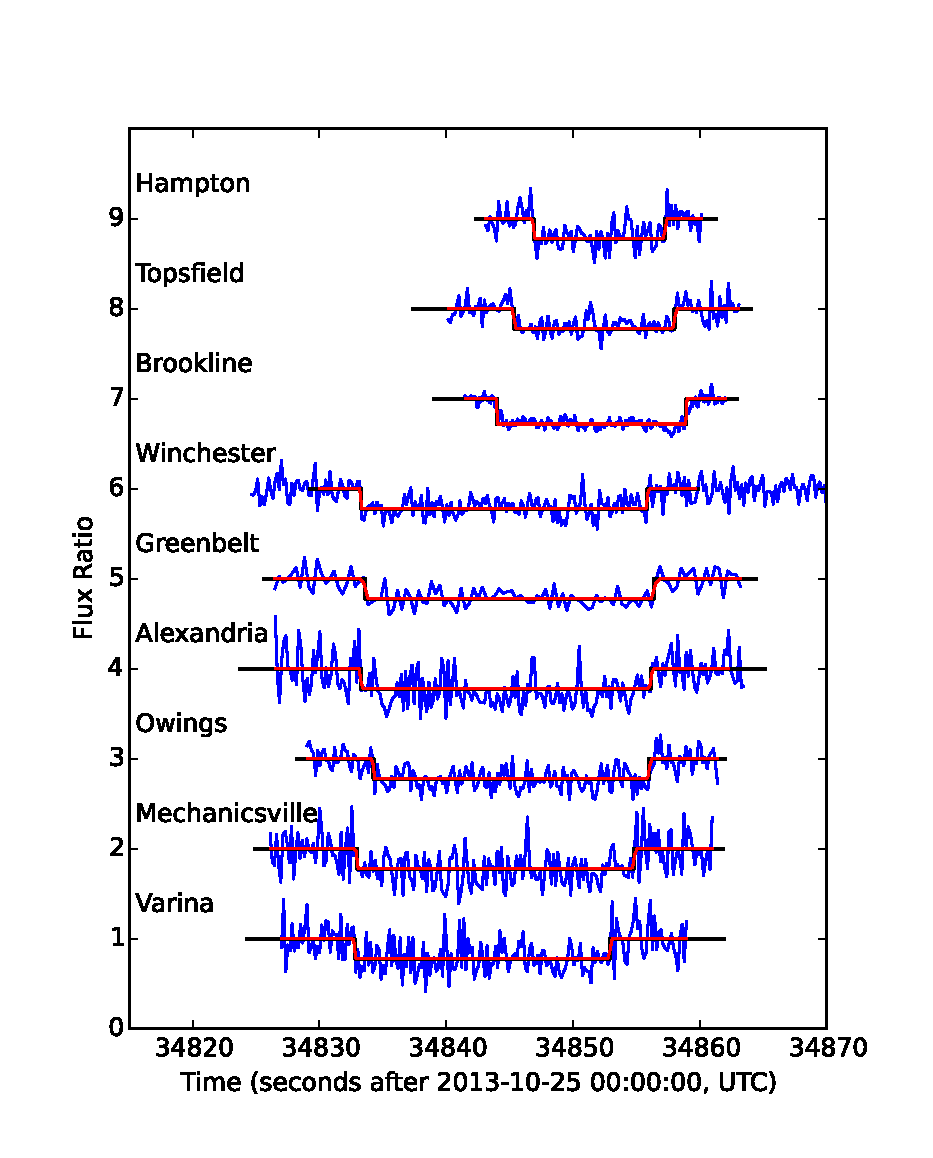
\includegraphics[scale=0.58]{figures/Ceres_2013_fluxratio.eps} 
\caption{The nine occultation light curves normalized and vertically shifted by a factor of 1.0 for better viewing, see Fig.~\ref{Fig: Ceres-2010-curves} for the explanation of the graph.% The solid black lines are the best fit of the square-well model to the data. The red lines are the square-well model convoluted with the Fresnel diffraction, the star diameter, and the applied exposure time. The mid-times of the occultations do not coincide due to the propagation delays of the shadow due to the distinct longitude of the sites. 
The light curve of Brookline is shifted by -64 s as explained in the text. \label{Fig: Ceres-2013-curves}}
\end{figure}




\subsection{Limb fitting solutions}

Elliptic limb profiles were adjusted to all the available\footnote{Brookline's chord was not used for limb fitting since it had an inaccurate absolute time.} chords by the same procedure described in Section \ref{Sec: limbfittingmethod}.%\footnote{For this event, the JPL\#33 Ceres' ephemeris was used to obtain the $f_{c}$ and $g_{c}$ coordinates.}
This yielded $\chi^2_{r,min} = 13$, suggesting that an elliptic model is not satisfactory to the data. Indeed, a quick glance at a plot of the observed chords, such as in Fig. \ref{Fig: Ceres-2013-body}, shows that the Varina chord seems to be somewhat advanced with respect to the others. Taking into account that in this station time stamps were not inserted on the video frames, it is fairly possible to attribute this advance to an eventual problem on the correspondence between camcorder's and GPS' times. This could be caused, for example, if the camcorder delayed to start the recording and, since this was an unattended pre-pointed station, this fact would not be noticed by the analysis of the video itself.

The immersion recorded at Owings also seems to be shifted (delayed) with respect to the nearby chords (see Fig. \ref{Fig: Ceres-2013-body}). This chord, actually, has roughly the same length of Mechanicsville's, despite the fact that they are separated by about 100 km. Differently from Varina, though, this station had time stamps inserted in each frame of the video, which makes it more unlikely to justify an eventual timing issue. Another possible explanation for the apparent problem of the times of this chord is the determination of the ingress and egress instants in the light curve analysis, which could have been affected by noise. Finally, the delay during the ingress could be caused by a relief feature in Ceres; we shall soon return to this hypothesis.

In a second limb fitting, thus, we did not consider Brookline, Varina and Owings chords. The adjust of the five parameters which define an ellipse to the 12 contacts then resulted in $\chi^2_{r,min} = 1.27$, indicating that the fitting is in good agreement with the observed data within the error bars. This is the solution depicted in Fig.~\ref{Fig: Ceres-2013-body}, where we see that the chord length measured in Brookline is compatible to the model. The associated physical parameters are presented in Table~\ref{Tab: results} as the nominal solution.

For this event the polar aspect angle is $\zeta = 90.7\degr$, which makes the true oblateness equal to the apparent one, within the error bars.

The position angle of this nominal solution is better constrained than the 2010 occultation. Actually, the uncertainty in the former is of $5\degr$ in contrast to $10\degr$ of the latter. This suggests that the pole-constrained solution obtained via the position of Ceres' pole (Eq. \ref{Eq: Pole}) would not be significantly different from the nominal one.

This assumption was confirmed when we carried out the limb fitting with the constraint $P = (25 \pm 3)\degr$, the position angle at the occultation which follows from Eq. \ref{Eq: Pole}. The physical parameters related to this pole-constrained solution are presented in the last column of Table~\ref{Tab: results}, and are essentially the same of the nominal solution.

In the hypothesis that the delay observed in the immersion at Owings could be associated to a limb topography feature, the recorded contact would then correspond to a negative elevation of 31 $\pm$ 4 km with respect to the best-fitting ellipse. Theoretical models, however, predict that reliefs in Ceres should not be higher than about 10--20 km \citep{Johnson1973}, while published observational data sets the bound of 18 km \citep{Carry2008}. More recently, images by the probe \textit{Dawn} also reveal an even smoother surface. Therefore, the association of Owings first contact to a relief is improbable.

\begin{figure}
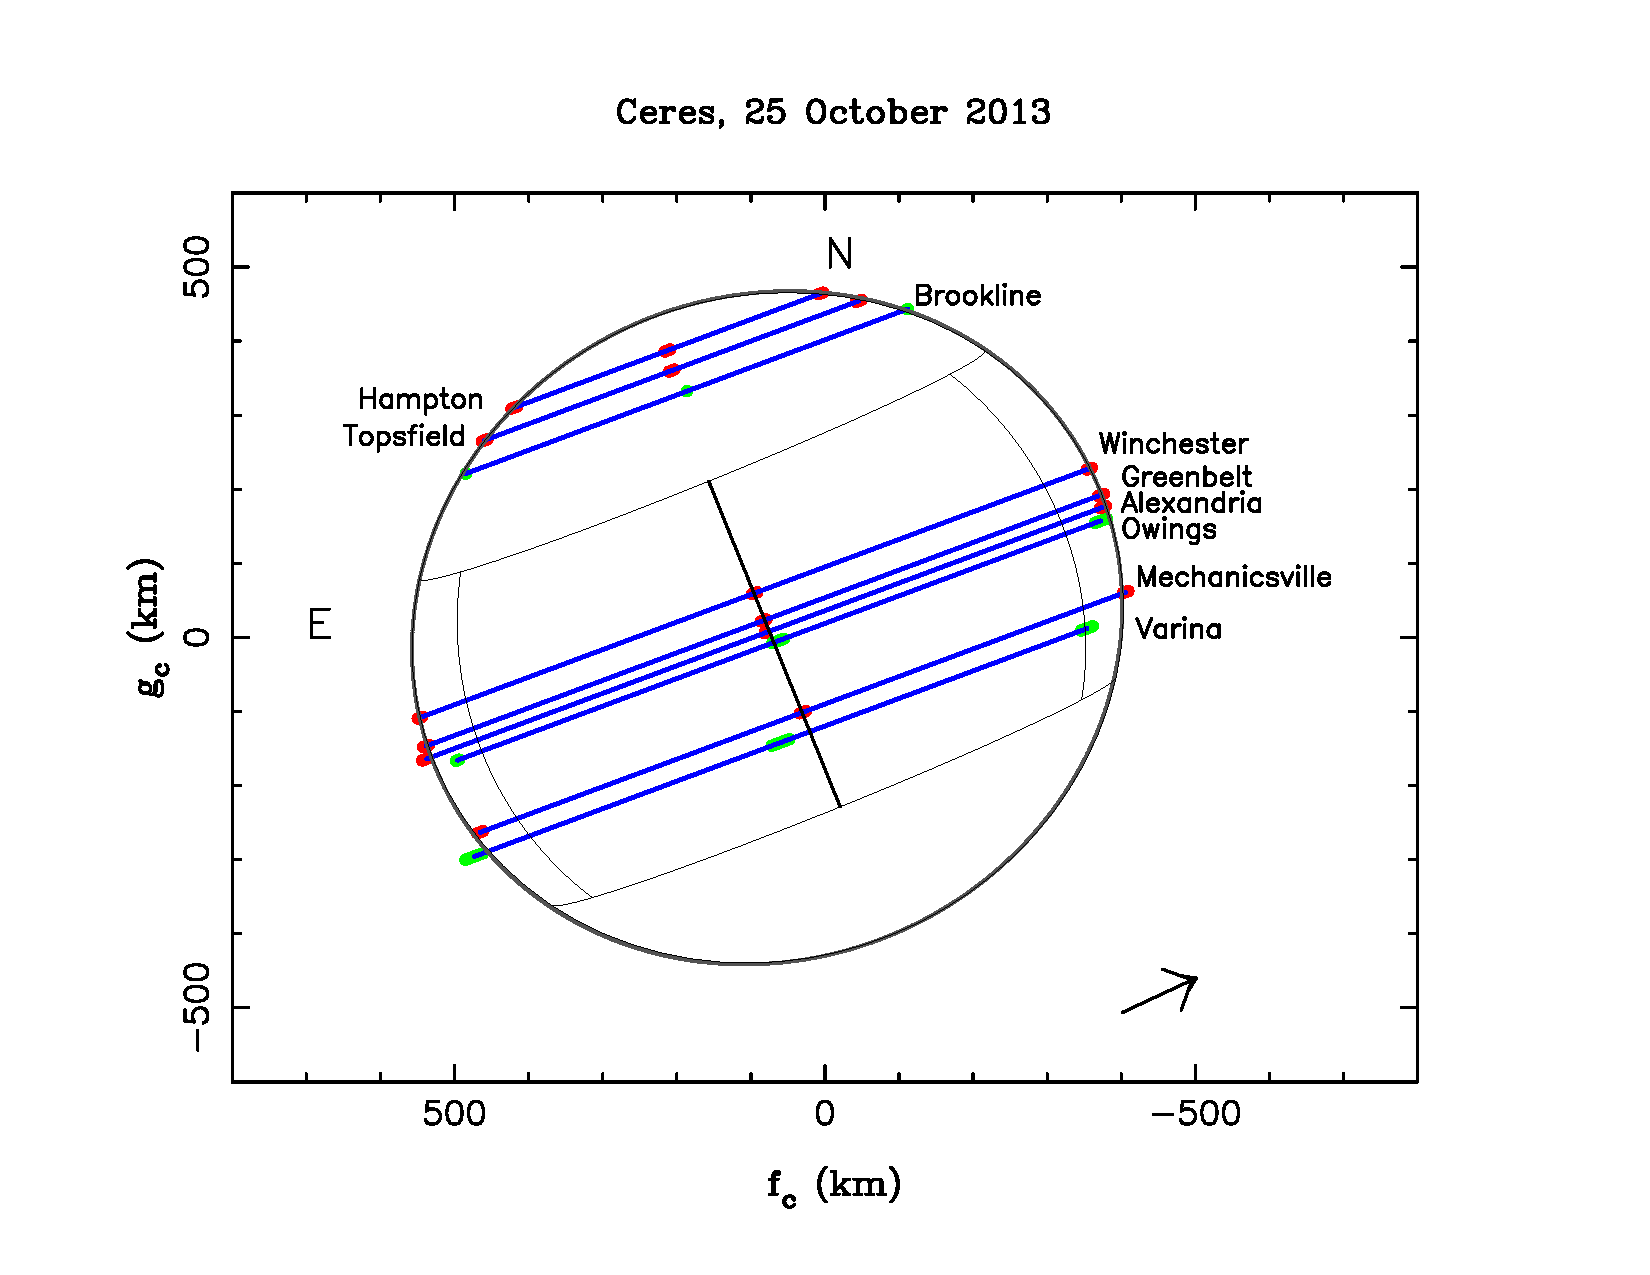
\includegraphics[scale=0.36]{figures/Ceres_2013_sphere.pdf}
\caption{The best elliptical fit for the occultation chords for the event of 2013 using timing from Table \ref{Tab: obs-2013} and the pole-constrained solution.  The arrow indicates the direction of motion, blue lines are the observed chords, the red and green segments are the ingress, egress and mid-occultation error bars at 1-$\sigma$ level. The chords with green error bars were not used during the limb fit process. The chord of Brookline if shifted by -64s as explained in the text.\label{Fig: Ceres-2013-body}}
\end{figure}


\section{Astrometry from Occultations}

The objects' geocentric positions derived from stellar occultations are most valuable for improving their orbits \citep{Desmars2015}. Usually the precision of the astrometric positions are limited by the accuracy of the occulted star position, not by the limb fit. Ceres' geocentric J2000 positions at the time of each occultation are displayed in Eqs.~\ref{Eq: Ceres-2010_pos} and \ref{Eq: Ceres-2013_pos}. The errors of the positions come from the errors of the star positions, taken from the catalogues and from the errors of the relative apparent distances between star and Ceres, derived from the limb fit (which are displayed as $\Delta\alpha \cos\delta$, $\Delta\delta$).

%\caption{Ceres' geocentric positions from the reported stellar occultations \label{Tab: Ceres-astrometry}}
\begin{equation}
2010 ~ \text{Aug} ~ 17
\left\{
 \begin{array}{l l}
    \text{Time} = 22:40:00\\
    \alpha = 17^{\rmn{h}}18^{\rmn{m}}29\fs0122\pm0\farcs027\\
    \delta = -27\degr 26\arcmin 38\farcs617\pm0\farcs028\\
    \Delta\alpha\cos\delta = 0\farcs003; ~~\Delta\delta = 0\farcs007
  \end{array}
\right.
\label{Eq: Ceres-2010_pos}
\end{equation}
\begin{equation}
2013 ~ \text{Oct} ~ 25
\left\{
  \begin{array}{l l}
    \text{Time} = 09:45:00\\
    \alpha = 11^{\rmn{h}}57^{\rmn{m}}52\fs9154\pm0\farcs019\\
    \delta = +09\degr 07\arcmin 49\farcs865\pm0\farcs021\\
    \Delta\alpha\cos\delta = 0\farcs002; ~~\Delta\delta = 0\farcs007
  \end{array}
\right.
\label{Eq: Ceres-2013_pos}
\end{equation}




\section{Discussion}

A quick glance at Table~\ref{Tab: results} shows an overall agreement between the physical parameters derived from both occultations, specially in the equatorial diameter. The differences of the solutions occur basically on the size of their error bars, and can be justified by the particularities of each set of data, as discussed below. 

The 2010 event, for example, had only seven contacts; none the less, they were well distributed over Ceres' disc (see Fig. \ref{Fig:Ceres-2010-body}) acting as a constraint to its shape. On the other hand, the 2013 event had five more exploitable contacts, but they were concentrated in certain regions of the body. In particular, the absence of chords close to Ceres' south pole made its oblateness worse determined here than in the 2010 event.

However, even our best measurement for the oblateness, $\epsilon=0.08 \pm 0.03$, has still a higher uncertainty with regard to other figures published in the literature, as Table~\ref{Tab: Ceres-final} shows. A larger number of uniformly spaced chords would be necessary to offer a best constraint to the oblateness. 

The few chords of the 2010 occultation could themselves only constraint the position angle of the object to a uncertainty of $10\degr$. This uncertainty was reduced by a factor of two in the 2013 event, approaching --and verifying-- the result predicted by the work of \cite{Drummond2014}. As was shown, using the coordinates of Ceres' polar axis to limit the position angle was not an efficient procedure in the 2013 event, in the sense that it did not result in significant changes in the parameters obtained in the nominal solution (see Table \ref{Tab: results}).

On the other hand, constrain the position angle on the 2010 occultation was proved to reduce the error bars of the other parameters (disregarding oblateness). Moreover, this procedure resulted in an excellent agreement between the equatorial radius figures of both events.

The 2013 occultation, therefore, offers not only an independent verification of the figures resulted from the 2010 event, but also validates the procedure carried out there which led to the best-constrained parameters in this work.

Comparison of Ceres' equatorial diameter as measured by different techniques is carried out in Table \ref{Tab: Ceres-final}. We note an overall agreement between our result to those obtained via direct imaging by the Hubble Space Telescope (HST) \citep{Thomas2005}, the Keck Observatory and the ESO VLT \citep{Drummond2014}. The smaller figure reported by \cite{Carry2008} may be justified by the fact that in this study the effects of limb-darking were not taken into account, as pointed out by \cite{Drummond2014}.

As mentioned in the Introduction, the 1984 event \citep{Millis1987} is the only occultation data to which we can compare our result. The measured diameters do not agree, ours being larger by 2-sigma. It is difficult to state for sure the reasons for this divergence since we had no access to the original 1984 data or reduction methodology. We note, however, that in this occultation a variation of 0.5 s in the contact times correspond to almost 7 km on Ceres' limb, which is on the same order of the residuals of their elliptical fit. Therefore, in order to properly compare their result to ours it would be necessary to reduce their light curves with the same methodology used in the present work.

NASA's \textit{Dawn} mission shall bring light to these questions, which will be important not only for the knowledge of Ceres itself, but also for all the techniques used so far to study the physical properties of small Solar System objects, such as the stellar occultations.

\begin{table}
  \caption{Ceres' equatorial diameter and oblateness \label{Tab: Ceres-final}}
  \begin{centering}
  \begin{tabular}{@{}lccc}
  \hline
     Eq. diameter (km) & Oblateness & Method & Ref. \\
\hline
$972 \pm 6$  & $0.08  \pm 0.03$  & Occultation & 1\\
$967 \pm 10$ & $0.078 \pm 0.015$ & Keck+VTL    & 2 \\
$959 \pm 5$  & $0.074 \pm 0.007$ & Keck        & 3\\
$975 \pm 4$  & $0.067 \pm 0.005$ & HST         & 4\\
$959 \pm 5$  & $0.05  \pm 0.01$  & Occultation & 5\\
\hline
\end{tabular}
\par\end{centering}
\textbf{References.} 1: Present work. 2: \cite{Drummond2014}. 3: \cite{Carry2008}. 4: \cite{Thomas2005}. 5: \cite{Millis1987}.
\end{table}




\section*{Acknowledgements}

ARGJ thanks the financial support of CAPES. BLG thanks CNPq. F.B.R. acknowledges PAPDRJ-FAPERJ/CAPES E-43/2013 number 144997, E-26/101.375/2014 and CDFB-CAPES/Brazil. M.A. acknowledges CNPq grants 473002/2013-2, 482080/2009-4 and 312394/2014-4, and FAPERJ grant 111.488/2013. RVM thanks grants: CNPq-306885/2013, Capes/Cofecub-2506/2015, Faperj/PAPDRJ-45/2013. J.I.B. Camargo acknowledges CNPq for a PQ2 fellowship (process number 308489/2013-6). We also acknowledge Steve Preston for the predictions of the occultations.


\begin{thebibliography}{99}

\bibitem[\protect\citeauthoryear{Assafin et al.}{2011}] {2011gfun.conf...85A} Assafin M., et al., 2011, in Tanga P., Thuillot W., eds, Gaia follow-up network for the solar system objects: Gaia FUN-SSO workshop proceedings. IMCCE-Paris Observatory, Paris, p. 85

\bibitem[\protect\citeauthoryear{Braga-Ribas et al.}{2013}]{BragaRibas2013} Braga-Ribas F. et al., 2013,
ApJ, 773, 26

\bibitem[\protect\citeauthoryear{Braga-Ribas et al.}{2014}]{BragaRibas2014} Braga-Ribas F. et al., 2014,
Nature, 508, 72

\bibitem[\protect\citeauthoryear{Carry et al.}{2008}] {Carry2008} Carry B. et al., 2008,
A\&A, 478, 235

\bibitem[\protect\citeauthoryear{Castillo-Rogez}{2011}]{CastilloR2011} Castillo-Rogez J.~C.,
2011, Icarus, 215, 599 

\bibitem[\protect\citeauthoryear{Desmars et al.}{2015}]{Desmars2015} Desmars J. et al., 2015, A\&A, submitted

\bibitem[\protect\citeauthoryear{Drummond et al.}{2014}]{Drummond2014} Drummond J.D. et al., 2014,
Icarus, 236, 28

\bibitem[\protect\citeauthoryear{Dunham et al.}{2014}]{Dunham2014}
Dunham D.W. et al., 2014, Asteroid Occultations V12.0. EAR-A-3-RDR-OCCULTATIONS-V12.0. NASA Planetary Data System

\bibitem[\protect\citeauthoryear{Gomes et al.}{2005}]{Gomes05} Gomes R., Levison H.~F., Tsiganis K., Morbidelli A.,\ 2005, Nature, 435, 466 

\bibitem[\protect\citeauthoryear{Giorgini et al.}{1996}]{Giorgini1996} Giorgini, J. D. et al., 1996, BAAS, 28, 1158

%\bibitem[\protect\citeauthoryear{Hog et al.}{2000}] {Hog2000} Hog E. et al., 2000,
%A\&A, 355, L27

\bibitem[\protect\citeauthoryear{Johnson \& McGetchin}{1973}] {Johnson1973} Johnson T.V., McGetchin T.R., 1973,
Icarus, 18, 612

\bibitem[\protect\citeauthoryear{K\"{u}ppers et al.}{2014}]{Kuppers2014} K\"{u}ppers M. et al., 2014,
Nature, 505, 525

\bibitem[\protect\citeauthoryear{McKinnon}{2012}]{McKinnon12} McKinnon W.~B.,\ 2012, LPI 
Contributions, 1667, 6475 

\bibitem[\protect\citeauthoryear{Millis et al.}{1987}]{Millis1987} Millis R.L. et al., 1987,
Icarus, 72, 507

%\bibitem[\protect\citeauthoryear{Ortiz et al.}{2012}]{Ortiz2012} Ortiz J.L. et al., 2012,
%Nature, 491, 566

\bibitem[\protect\citeauthoryear{Russell et al.}{2004}]{Russell2004} Russell C.~T. et al.,\ 2004, P\&SS, 52, 465 


\bibitem[\protect\citeauthoryear{Sicardy et al.}{2011}]{Sicardy2011} Sicardy B. et al., 2011,
Nature, 478, 493

\bibitem[\protect\citeauthoryear{Thomas et al.}{2005}]{Thomas2005} Thomas P.C. et al., 2005,
Nature, 437, 224

%\bibitem[\protect\citeauthoryear{van Belle}{1999}] {vanBelle1999} van Belle G.T., 1999,
%PASP, 111, 1515

\bibitem[\protect\citeauthoryear{Widemann et al.}{2009}] {Widemann2009} Widemann T. et al., 2009,
Icarus, 199, 458

%\bibitem[\protect\citeauthoryear{Zacharias et al.}{2004}]{Zacharias2004} Zacharias N. et al., 2004,
%AJ, 127, 3043

\bibitem[\protect\citeauthoryear{Zacharias et al.}{2013}]{Zacharias2013} Zacharias N. et al., 2013,
AJ, 145, 44



\end{thebibliography}



%\bsp

\label{lastpage}

\end{document}